\documentclass[10pt]{scrartcl} 

\usepackage[a4paper,left=1.5cm,right=1.5cm,top=2cm,bottom=2cm,bindingoffset=5mm]{geometry}

%% allgemeine Imports, die nicht mehr erforderlich sind, da ich mit lulatex kompiliere
% \usepackage[utf8x]{inputenc} % Zeichenkodierung
% \usepackage[ngerman]{babel}  % u.a. Silbentrennung
% \usepackage[T1]{fontenc}

%\usepackage{floatflt} 
%\usepackage{times}

%\usepackage{amsmath} %Bei Bedarf: Formeln
\usepackage{graphicx}   % Bilder
\graphicspath{{./image/}{./plantuml/}{./}}
%\begin{figure}[htbp] 
%	\centering
%	\includegraphics[width=3cm]{JavaSpringInitializr.png}
%	\caption{Logo}
%	\label{fig:Bild1}
%\end{figure}



\usepackage{wrapfig}
%\begin{wrapfigure}{l}{0.25\textwidth}
%	\centering
%	\includegraphics[width=0.25\textwidth]{contour}
%\end{wrapfigure}

%\usepackage{lastpage}
\usepackage{hyperref}
\usepackage{cclicenses}

%\usepackage{blindtext}  %% Zum Debugging: Blindtext einfügen

%%% zur Darstellung von Quellcode
\usepackage{listings}
\usepackage{color}
\usepackage{xcolor}

%%% Für individuelle Kopfzeilen
% https://esc-now.de/_/latex-individuelle-kopf--und-fusszeilen/?lang=en
%%%%%%%%%%%%%%%%%%%%%%%%%%%
\usepackage[headsepline=0.5pt,footsepline=0.5pt,plainheadsepline=true, plainfootsepline=true,headwidth=(\the\textwidth), footwidth=(\the\textwidth)]{scrlayer-scrpage}

% Alle Inhalte löschen.
\clearpairofpagestyles

%\renewcommand{\familydefault}{\sfdefault}

% Schriftformatierung zurücksetzen.
\setkomafont{pageheadfoot}{}
\setkomafont{title}{\bfseries}

% Linien einfärben.
\addtokomafont{headsepline}{\color{gray}}
\addtokomafont{footsepline}{\color{gray}}

% Statische Inhalte.
\ihead{\thetitle}
%\chead{Mitte oben}
\ohead{
	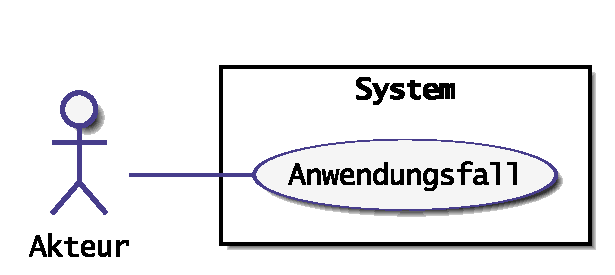
\includegraphics[height=1cm]{logo}	
}


% Unterschiedliche Inhalte für gerade/ungerade.
\ifoot*{\href{https://creativecommons.org/licenses/by/4.0/}{\ccby CC BY 4.0}, Hannes Stein  }
\cfoot*{\today}
\ofoot*{\pagemark}
\renewcommand*{\pagemark}{{\usekomafont{pagenumber}{Seite \thepage\ von \pageref*{LastPage}}}}


%\usepackage{showframe} % for debug information
\usepackage{titling}
\pretitle{
	
\begin{tabular}[b]{p{11cm} p{5cm}}
      \bfseries
		\LARGE
		\selectfont
		}
\posttitle{
 & 	
 \raisebox{-\height}{
 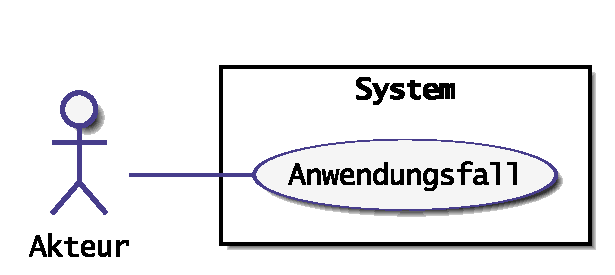
\includegraphics[width=4.5cm]{logo}
}
	\end{tabular}
}
%\preauthor{}\postauthor{}
\predate{}\date{}\postdate{}


%%%%%%%%%%%%%%%%%%%%%%%%%


%%% zur Darstellung von Quellcode
\definecolor{dkgreen}{rgb}{0,0.6,0}
\definecolor{gray}{rgb}{0.5,0.5,0.5}
\definecolor{lightgray}{rgb}{0.83, 0.83, 0.83}
\definecolor{mauve}{rgb}{0.58,0,0.82}

\lstset{
	frame=tb,	
	aboveskip=3mm,
	belowskip=3mm,
	columns=fixed,
	basicstyle={\small\ttfamily},
	numbers=left,
	numberstyle=\tiny\color{gray},
	firstnumber=last,
	keywordstyle=\color{blue},
	commentstyle=\color{dkgreen},
	stringstyle=\color{mauve},
	breaklines=true,
	breakatwhitespace=true,
	tabsize=3,
	includerangemarker=true,
	showtabs=false,
	showspaces=false
}

\lstdefinestyle{java}{
	language=Java,
	numbers=left, stepnumber=1, numberstyle=\tiny, numbersep=10pt}
\lstdefinestyle{bashquery}{
	language=bash,
	numbers=left,
	stepnumber=1,
	numberstyle=\tiny,
	numbersep=10pt}
\lstdefinestyle{response}{
	frame=trbl,
	aboveskip=0mm,
	belowskip=3mm,
	basicstyle={\scriptsize\ttfamily},
	frame=shadowbox, 
	rulecolor=\color{lightgray},
	rulesepcolor=\color{lightgray},
	numbers=none
}

\lstdefinestyle{nonumbers}{
	numbers=none
}

\lstdefinestyle{plantuml}{
	numbers=left, stepnumber=1, numberstyle=\tiny, numbersep=10pt,
	morekeywords=[1]{actor, usecase, rectangle, as},
	morekeywords=[2]{skinparam, ArrowColor, BorderColor, BackgroundColor},
	morekeywords=[3]{DefaultFontName},
	morekeywords=[4]{whitesmoke, DarkSlateBlue, LightYellow},
	morekeywords=[5]{note, top, on, link, end, left to right, direction, up, down},
	otherkeywords={ :,  .., .,  -, --, ->, -->, -|>, --|>, <-, <--, <|-, <|--, <., <.., <|., <|.., \\n, \{, \}} ,
	morecomment=[l]{'}
	}


%\hypersetup{
%	pdftitle    = { hihihi },
%	pdfsubject  = {Um was geht es },
%	pdfauthor   = {Autor bzw. Autoren},
%	pdfkeywords = {Stichwort1, Stichwort2 ...} ,
%	baseurl = {http://www.csbme.de},
%	pdfdisplaydoctitle = true
%}


\title{UML Anwendungsfall- (UseCase-) Diagramm
	 mit plantUML
 }
%\author{Hannes Stein}





\begin{document}
	\setlength{\droptitle}{-40pt} % lower the title
	\maketitle
%	\begin{abstract}
%	Wie interagiert ein (Software-)System mit dem Benutzer?
%	\end{abstract}

	

%\pagenumbering{roman}\setcounter{page}{1}
% \tableofcontents
% \listoffigures
% \listoftables



\pagenumbering{arabic}\setcounter{page}{1}

\section{Akteurinnen und Anwendungsfälle}

Ein Anwendungsfalldiagramm (\textit{UseCase}) beschreibt \textit{wie} ein (Software)-System mit Anwenderinnen\footnote{Grundsätzlich: es wird die feminine gramatikalische Form gewählt, maskuline Akteure sind immer \hyperref{https://twitter.com/hashtag/mitgemeint?lang=de}{}{}{\#mitgemeint}} interagiert. Es beschreibt, welche Anwendungsfälle ein System anbietet. Die Reihenfolgen oder Abläufe der Anwendungsfälle müssen jedoch auf andere Art modelliert werden. \\ 
Anwendungsfalldiagramme helfen v.a. dabei, die Vollständigkeit und Korrektheit des Systemverständnisses der Projektbeteiligten (Kunden, Fachdomäne, Entwicklerinnen) abzugleichen.

\begin{tabular}[b]{p{7cm} p{10cm}}
	
\raisebox{-\height}{
			
	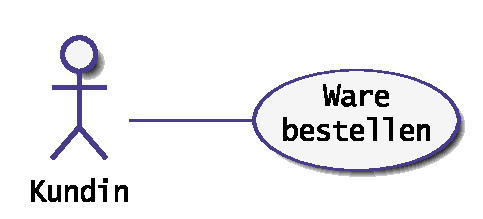
\includegraphics[width=6.5cm]{01_Bestandteile_UseCase.eps}
}
&
\begin{lstlisting}[style=plantuml]
@startuml 'Muss immer am Anfang stehen
 'Generell zum Lesen von Use-Case-Diagrammen einfacher:
 left to right direction

 'Akteurin festlegen 
 actor :Kundin: as customer

 ' UseCase definieren (mit Zeilenumbruch \n=Newline)
 usecase (Ware \n bestellen) as bestellen

 customer -- bestellen	 
@enduml
\end{lstlisting}
\end{tabular}
\textbf{Akteurinnen} sind Menschen oder andere Systeme, die Anwendungsfälle des Systems nutzen. Sie können auch Rollen (Kundin) oder Typen zusammenfassen. Sie werden in der Regel als Strichmensch (\textit{stick man}) notiert.
\\
Mit einem \textbf{Anwendungsfall (Use Case)} erzeugt das modellierte System erkennbaren Nutzen für die zugeordneten Akteurinnen. Ein Anwendungsfall fasst Aktionen zusammen, die (funktionale) Anforderungen erfüllen. Anwendungsfälle werden in der Regel als Ellipse notiert.
\\\textbf{Assoziationen} verbinden Anwendungsfälle mit den auslösenden oder benötigten Akteurinnen. Sie werden mit durchgezogenen Linien notiert.

\section{Systemgrenzen und Systemname}
\begin{tabular}[b]{p{7cm} p{10cm}}
%	\vspace{0cm}
\raisebox{-\height}{
		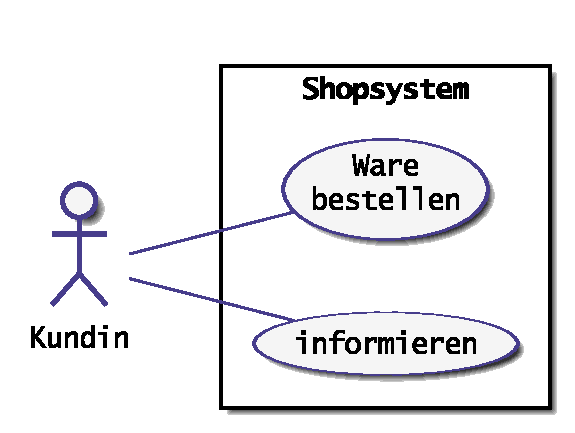
\includegraphics[width=6.5cm]{02_Systemgrenzen}
	}
	& 	

\begin{lstlisting}[style=plantuml]
actor :Kundin: as customer

'Definition der Systemgrenze über rectangle{}
rectangle Shopsystem {

	usecase (Ware \n bestellen) as bestellen

	'Kurzform ohne Deklaration des UseCases:
	customer -- (informieren)

	customer -- bestellen
}
\end{lstlisting}

 \end{tabular}
\\Die \textbf{Systemgrenze} legt fest, welche Anwendungsfälle im modellierten System enthalten sind. Das abgegrenzte System trägt einen Namen und spannt einen Namensraum auf.
\\Alle \textbf{Akteurinnen} stehen außerhalb der Systemgrenzen - andernfalls wären sie als Teil des Systems nicht gesondert zu modellieren. 
\\Systemgrenzen müssen nicht zwingend angegeben werden, dienen aber dem Verständnis und der Abgrenzung von Akteurinnen, Anwendungsfällen und externen Systemen.

\section{Vererbung von Akteuren und "oder"-Beziehungen}
Mit Hilfe von Vererbungsbeziehungen können Akteurinnen spezialisiert werden: Im Beispiel unten ist die Prokuristin eine spezielle Mitarbeiterin, der zusätzlich zu allen Anwendungsfällen einer Mitarbeiterin auch noch über eigene Anwendungsfälle verfügt. Vererbung wird - wie in der UML üblich - mit einer geschlossenen Pfeilspitze symbolisiert:
\begin{tabular}[b]{p{7cm} p{10cm}}
	
	\raisebox{-\height}{
			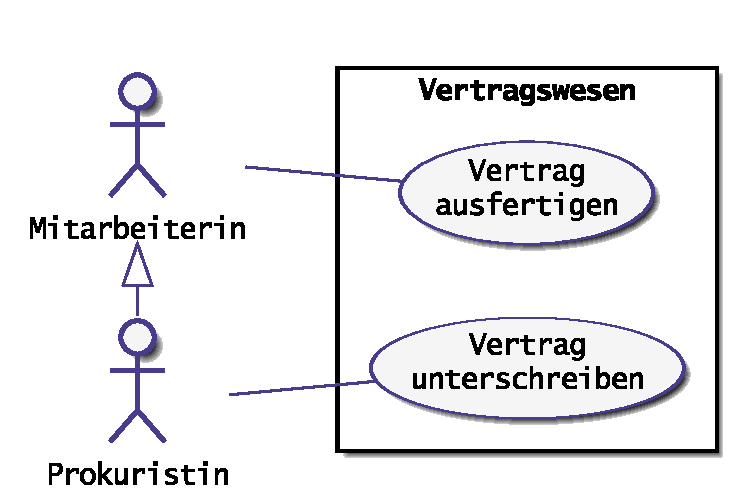
\includegraphics[width=6.5cm]{03_VererbungVonAkteuren}
	}
&
\begin{lstlisting}[style=plantuml] 
actor :Mitarbeiterin: as mitarbeiter
actor :Prokuristin: as prokurist

rectangle Vertragswesen {
	usecase (Vertrag \n ausfertigen) as ausfertigen
	usecase (Vertrag \n unterschreiben) as unterschreiben

	'Kurzform ohne Deklaration des UseCases:
	mitarbeiter -- ausfertigen
	prokurist -- unterschreiben
	mitarbeiter <|- prokurist
}	 
\end{lstlisting}
\end{tabular}
\\Vererbungsbeziehungen werden auch genutzt, um ODER-Beziehungen zu modellieren: Eine Geschäftsführerin oder eine Prokuristin darf Verträge unterschreiben. Solche Zusammenhänge lassen sich nur über einen generalisierten Akteur (hier: Befugte) realisieren.

\begin{tabular}[b]{p{7cm} p{10cm}}
	
	\raisebox{-\height}{
		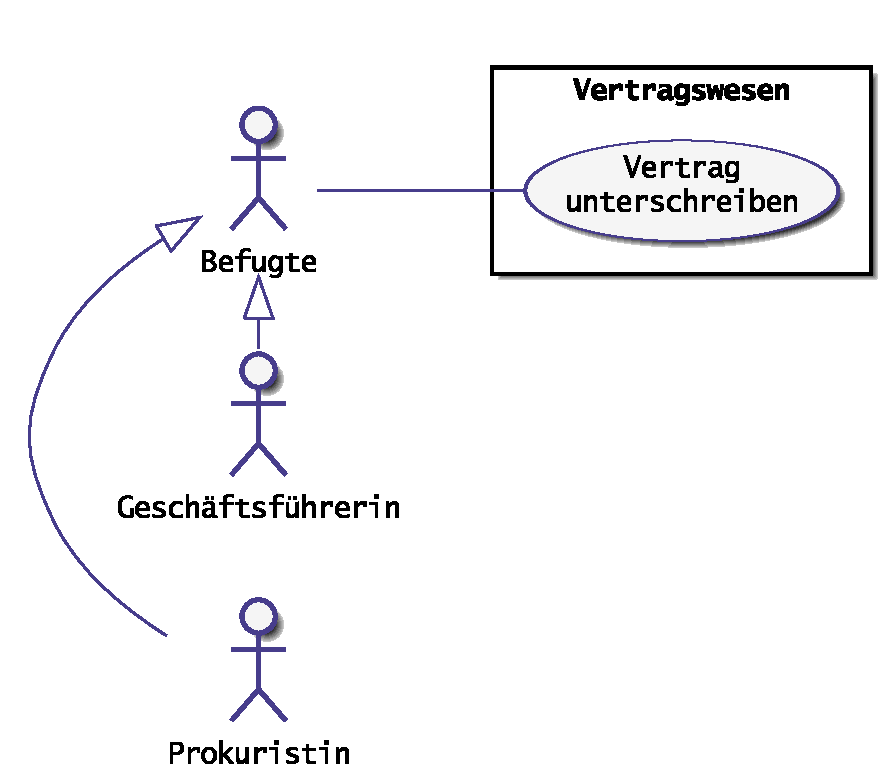
\includegraphics[width=6.5cm]{03_Vererbung_OderBeziehungenVonAkteuren}
	}
	&
	\begin{lstlisting}[style=plantuml] 
actor :Befugte: as befugte
actor :Prokuristin: as prokuristin
actor :Geschäftsführerin: as gf
	
rectangle Vertragswesen {
	usecase (Vertrag \n unterschreiben) as unterschreiben
	
	befugte -- unterschreiben
	befugte <|- prokuristin
	befugte <|- gf
}
	\end{lstlisting}
\end{tabular}
\\Akteurinnen, die zwar als Generalisierung anderer Rollen modelliert werden, die es aber konkret (als Instanz im OOP-Sinne) nie gibt, können als abstrakte Akteurinnen modelliert werden. Ihr Name wird kursiv geschrieben und/oder mit dem \textit{Constraint} \{abstract\} gekennzeichnet:

\begin{tabular}[b]{p{7cm} p{10cm}}
	
	\raisebox{-\height}{
		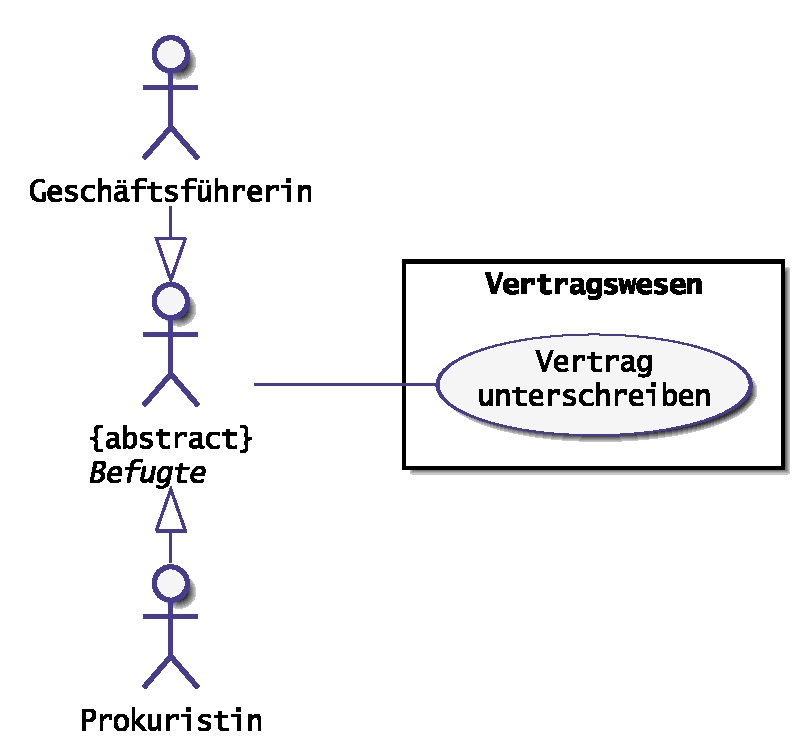
\includegraphics[width=6.5cm]{03_Vererbung_Abstrakt}
	}
	&
	\begin{lstlisting}[style=plantuml] 
actor :{abstract}\n<i>Befugte</i>: as befugte
actor :Prokuristin: as prokuristin
actor :Geschäftsführerin: as gf
	
rectangle Vertragswesen {
	usecase (Vertrag \n unterschreiben) as unterschreiben
	
	befugte -- unterschreiben
	befugte <|- prokuristin
	gf -|> befugte 
}
	\end{lstlisting}
Hier wurde ein Akteur oberhalb und einer unterhalb positioniert, in dem die Pfeilrichtung umgekehrt wurde.
\end{tabular}



\section{Anwendungsfälle, die weitere Anwendungsfälle immer beinhalten}
Sofern zur Erfüllung eines Anwendungsfalls in jedem Fall auf die Funktionalität eines zweiten Anwendungsfalls zurückgegriffen werden muss, kann dieser über eine \textit{include}-Beziehung verknüpft werden. Wichtig ist, dass der eingebundene Anwendungsfall auch isoliert einen abgeschlossenen Nutzen generiert (also nicht fester Bestandteil des anderen Anwendungsfalls ist). Diese "beinhaltet"-Beziehung wird durch eine gestrichelte Linie mit Pfeilspitze dargestellt, die in Richtung des einbezogenen Anwendungsfalls zeigt und die mit dem Stereotyp \guillemotleft include\guillemotright versehen wird. Der Pfeil kann als "beinhaltet" in Pfeilrichtung gelesen werden.
\\
\begin{tabular}[b]{p{7cm} p{10cm}}
	
	\raisebox{-\height}{
			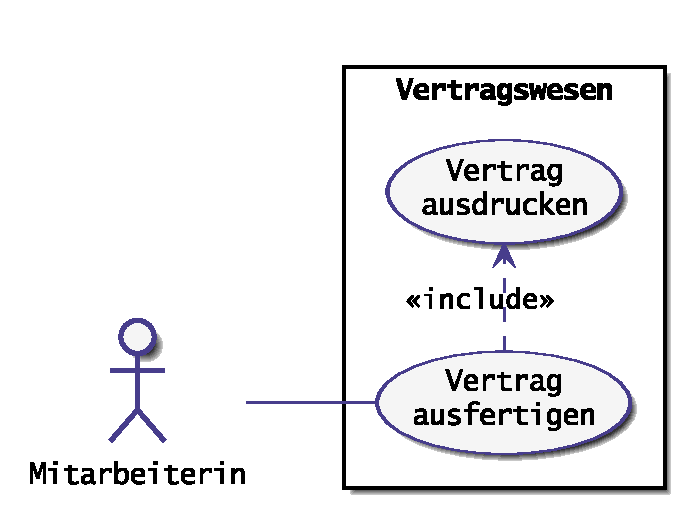
\includegraphics[width=6.5cm]{05_include}
	}
	&

\begin{lstlisting}[style=plantuml]
actor :Mitarbeiterin: as mitarbeiter

rectangle Vertragswesen {
	usecase (Vertrag \n ausfertigen) as ausfertigen
	usecase (Vertrag \n ausdrucken) as drucken

	mitarbeiter -- ausfertigen

	'Die gestrichelte Linie wird per .> angegeben
	'und das Stereotyp nach dem Doppelpunkt:
	ausfertigen .> drucken : <<include>>
} 
\end{lstlisting}
\end{tabular}
\\Die Gefahr ist groß über \textit{include}-Beziehungen Programmabläufe und Unterfunktionsaufrufe zu modellieren. Daher bitte immer prüfen: Stellt der inkludierte Anwendungsfall wirklich einen eigenständig auslösbaren Anwendungsfall dar?


\section{Anwendungsfälle, unter Umständen durch weitere Anwendungsfälle erweitert werden}
Sofern ein Anwendungsfall nur unter bestimmten Umständen um die Funktionalitäten eines zweiten Anwendungsfalls erweitert wird, werden beide über eine \textit{extend}-Beziehung verknüpft. Zu jeder \textit{extend}-Beziehung \textit{sollte} angegeben werden, unter welcher Bedingung (\textit{condition}) welcher Anwendungsfall erweitert wird.
Ein gestrichelter Pfeil zeigt vom erweiternden auf den zu erweiternden Anwendungsfall und ist mit dem Stereotyp \guillemotleft include\guillemotright versehen. An dieser Linie sollte eine Notiz mit \textit{condition} und \textit{extension point} notiert werden. Der  \textit{extension point} wird auch am Ursprungs-Anwendungsfall notiert. Der Pfeil kann als "erweitert" in Pfeilrichtung gelesen werden.
\\
\begin{tabular}[b]{p{7cm} p{10cm}}
	
	\raisebox{-\height}{
			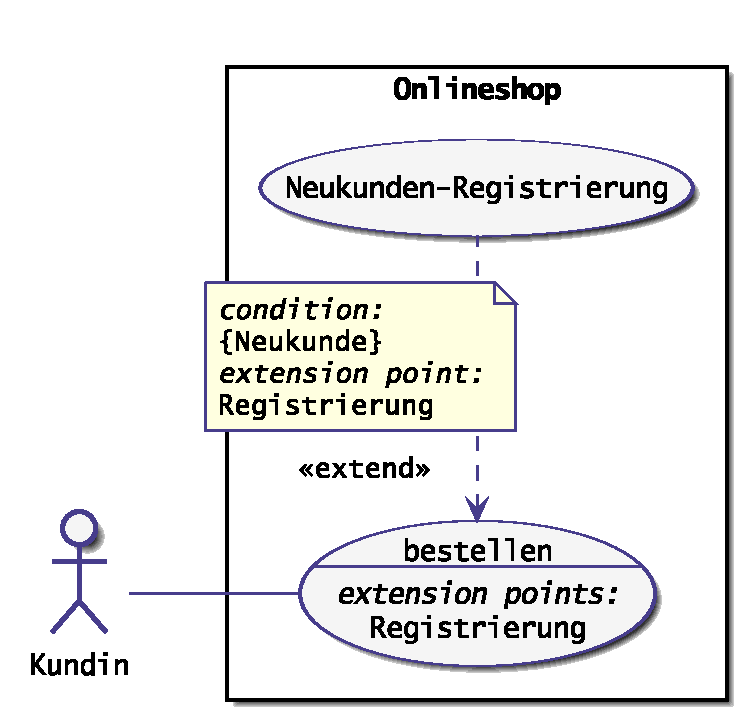
\includegraphics[width=6.5cm]{06_extend}
}

	&

\begin{lstlisting}[style=plantuml]
actor :Kundin: as customer

rectangle Onlineshop {
	'Angabe des extention point
	usecase bestellen as "bestellen
		--
		<i>extension points:</i>
		Registrierung"  

	customer -- bestellen

	'der Stereotyp 
	bestellen <.(Neukunden-Registrierung) : <<extend>>

	'condition und extension point
	note top on link
		<i>condition:</i>
		{Neukunde}
		<i>extension point:</i>
		Registrierung
	end note
}	 
\end{lstlisting}
\end{tabular}


\section{Vererbung von Anwendungsfällen}
Analog zu Akteurinnen können auch Anwendungsfälle spezialisiert werden. Beispielsweise kann ein generalisierter Anwendungsfall "Artikel kaufen" bestehen aus dem Szenario:
\\
1. Artikel in Warenkorb legen / 2. Warenkorb bestellen / 3. Kauf abwickeln
\\Die spezialisierten Anwendungsfälle ändern Details in den Szenarien, z.B. bei "Buch per Versand kaufen": 
\\1. Artikel in Warenkorb legen / 2. Warenkorb bestellen / 3a Versandadresse abfragen / 3b Bezahldetails abfragen
\\oder bei "eBook kaufen": 
\\1. Artikel in Warenkorb legen / 2. Warenkorb bestellen / 3. Paypal-Kaufabwicklung starten / 4. Downloadlink bereitstellen
\\Auch Anwendungsfälle kennen das konzept der Abstraktion: "Artikel kaufen" selbst kann nicht ausgeführt werden, sondern modelliert nur ein Gerüst, das in konkreten Anwendungsfällen noch ausformulieren müssen.
\\Die Notation entspricht der für Vererbung (geschlossene Pfeilspitze) und Abstraktion (kursive Schrift, \textit{constraint} \textit{\{abstract\}}) bekannten Darstellung.
\\
\begin{tabular}[b]{p{7cm} p{10cm}}
	
	\raisebox{-\height}{
			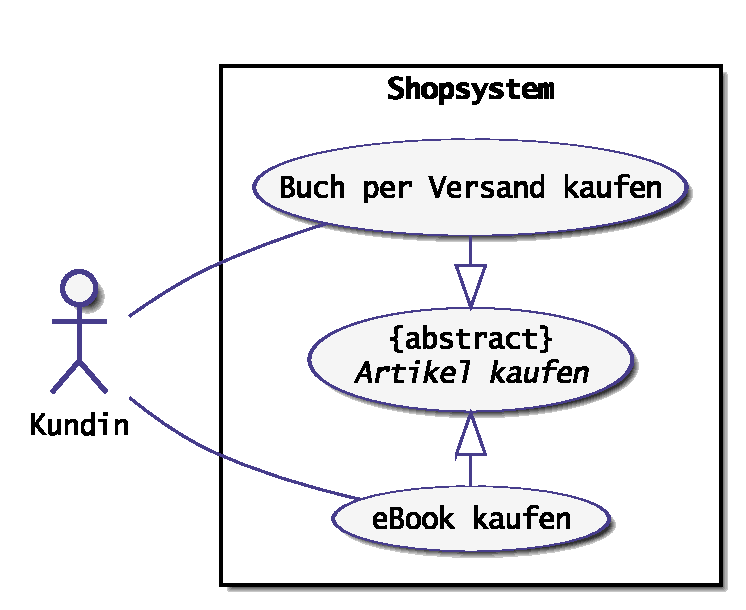
\includegraphics[width=6.5cm]{08_UseCaseVererbung}
	}
	&

\begin{lstlisting}[style=plantuml]
actor :backend: as backend

rectangle Shopsystem {
	usecase (Bestellung bearbeiten) as bestellung
	usecase (Online-Bestellung bearbeiten) as onlinebestellung

	bestellung <|-onlinebestellung
}	 
\end{lstlisting}

\end{tabular}

\section{Wie viele Akteurinnen stehen mit wie vielen UseCases in Beziehung?}
Um festlegen zu können, wie viele Akteurinnen für Anwendungsfälle nötig sind und an wie vielen Anwendungsfällen Akteurinnen beteiligt sind werden - analog zum UML-Klassendiagramm - Multiplizitäten angegeben, wie am Beispiel zu sehen:
\\An einem Tischtennis-Rundlauf sind mindestens 3 Spielerinnen beteiligt, jede Spielerin  jedoch an exakt einem Rundlauf-Spiel. An einem Rundlaufspiel kann eine Schiedsrichterin beteiligt sein. Jede Schiedsrichterin kann an keinem oder beliebig vielen Rundlaufspielen beteiligt sein:
\\
\begin{tabular}[b]{p{7cm} p{10cm}}
	\raisebox{-\height}{
		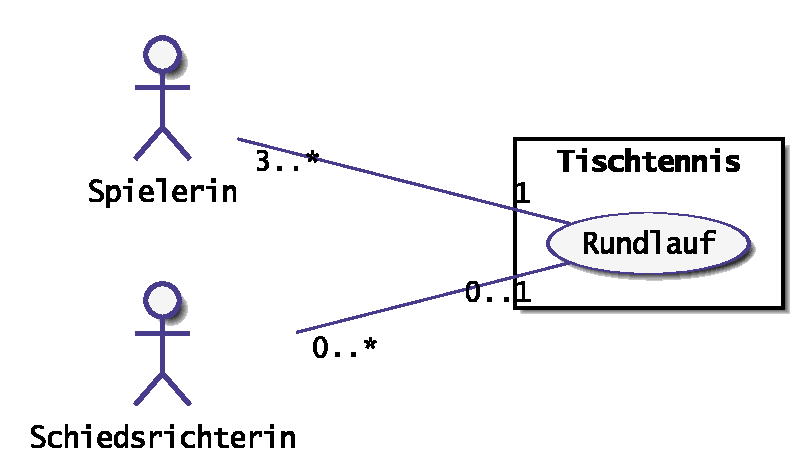
\includegraphics[width=6.5cm]{07_Multiplizitaeten}
	}
	&
	\begin{lstlisting}[style=plantuml]
actor :Spielerin: as player
actor :Schiedsrichterin: as referee

rectangle Tischtennis {
	usecase (Rundlauf) as rundlauf

	'Multiplizitäten werden an den Assoziationen angegeben
	player "3..*" --- "1" rundlauf
	referee "0..1" --- "0..*" rundlauf
}	  
	\end{lstlisting}
\end{tabular}
\\Da diese Information jedoch häufig für die Adressaten des Use-Case-Diagramms keine Rolle spielt werden Multiplizitäten eher selten notiert.

\section{Gerichtete Assoziationen (initiiernde und sekundäre Akteurinnen)}
In seltenen Fällen wir die Kommunikationsrichtung in Anwendungsfalldiagrammen dargestellt. So kann verdeutlicht werden, welche Akteurinnen den Anwendungsfall aktiv triggern (primäre Akteurinnen) und wer nur passiv vom Anwendungsfall benötigt wird (sekundäre Akteurinnen).
\\
\begin{tabular}[b]{p{7cm} p{10cm}}
	\raisebox{-\height}{
					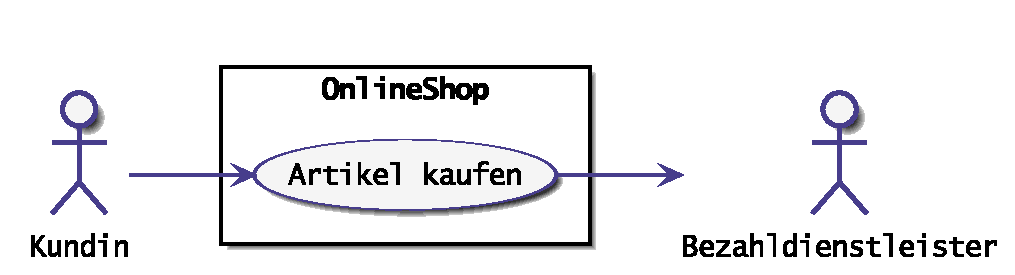
\includegraphics[width=6.5cm]{09_GerichteteBeziehungen}
	}
	&
\begin{lstlisting}[style=plantuml]
actor :Bezahldienstleister: as bezahl
actor :Kundin: as kundin
rectangle OnlineShop {
	usecase (Artikel kaufen) as kauf
}
kundin --> kauf
kauf --> bezahl
\end{lstlisting}
(Wenn left to right direction gewählt wurde muss der Akteur mit up positioniert werden.)

\end{tabular}

\section{plantUML-Formatierung: Ausrichtung der Linien durch einfache oder zweifache Zeichen (- / -- / . / ..)}

PlantUML bietet die Möglichkeit Assoziationsrichtungen vorzugeben über die Operantoren -up-, -down-, -left-, -down-. Wenn man jedoch die Programme mit der Option "left to right direction" nutzt sind durch die Drehung sämliche Richtungsanweisungen verkehrt...
\\Als Alternative kann man auch die Notation mit einfachen und doppelten Bindestrichen wählen:
\\
\begin{tabular}[b]{p{7cm} p{10cm}}
	
	\raisebox{-\height}{
		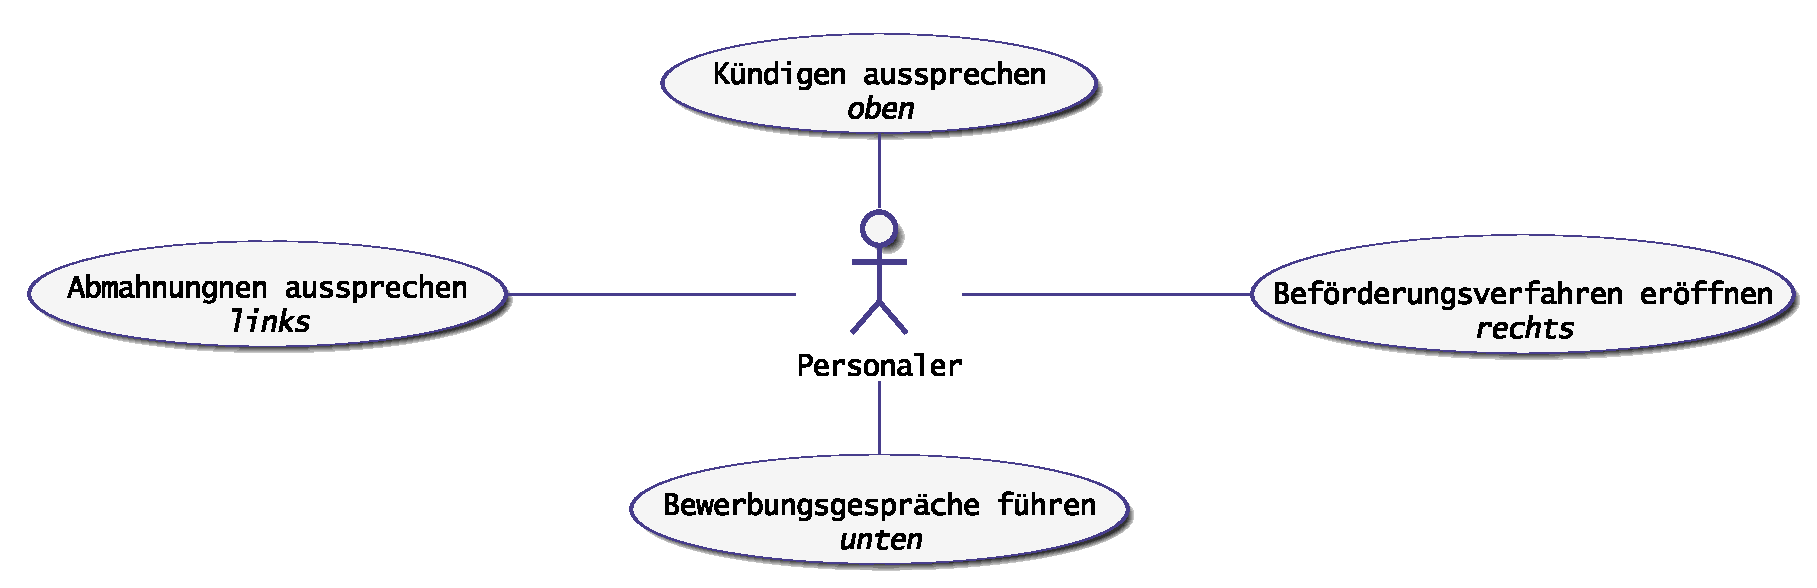
\includegraphics[width=6.5cm]{04_Ausrichtung}
	}
	&
	\begin{lstlisting}[style=plantuml]
'wie immer wurde die Richtung gedreht:
left to right direction

actor :Personaler: as personaler

'nach oben dann mit nur einem Bindestrich:
(Kündigen aussprechen \n <i> oben </i>)- personaler 

'nach unten durch vertauschen von Akteurin und UseCase
personaler - (Bewerbungsgespräche führen  \n <i> unten </i>)

'seitlich nach rechts mit zwei Strichen
personaler -- (Beförderungsverfahren eröffnen  \n <i> rechts </i>)

'seitlich nach links mit Vertauschten Positionen
(Abmahnungnen aussprechen \n <i> links </i>) -- personaler
	\end{lstlisting}
\end{tabular}

\section{plantUML-Formatierung: Aufhübschen von  Anwendungsfall-Diagrammen}

Wenn die Diagramme erstmal stehen will man sie aufhübschen. Dafür stehen allerlei möglichkeiten zur Verfügung, die v.a. auf der plantUML-Seite dargestellt werden. Einige Beispiele sind hier abgebildet:
\\
\begin{tabular}[b]{p{5.5cm} p{5.5cm} p{5.5cm}}
	\raisebox{-\height}{
	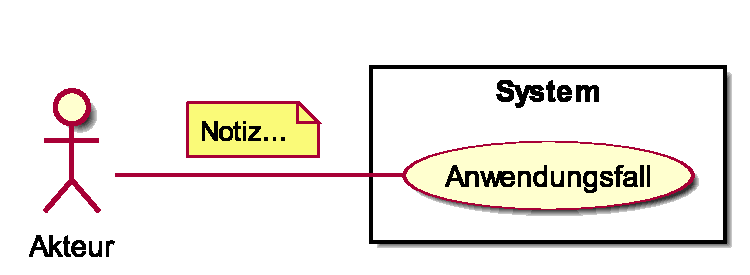
\includegraphics[width=5cm]{10_Aufhuebschen1}
}
Minimalbeispiel: nur die Leserichtung wurde angepasst:
&

\raisebox{-\height}{
	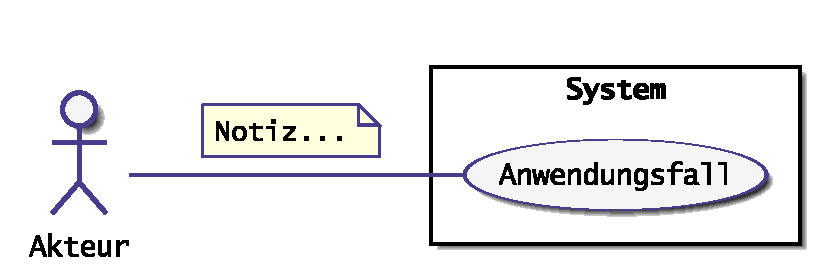
\includegraphics[width=5cm]{10_Aufhuebschen2}
}
Anpassung von Schriftart und Farben
& 
\raisebox{-\height}{
	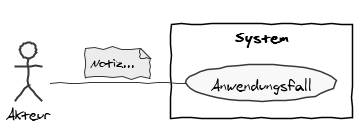
\includegraphics[width=5cm]{10_Aufhuebschen3}
} 

Sieht nach Entwurf aus: um die Vorläufigkeit und Änderbarkeit zu unterstreichen kann man es nach einer Skizze aussehen lassen.
\\

\begin{lstlisting}[style=plantuml]
@startuml

left to right direction

actor :Akteur:
rectangle System {
usecase Anwendungsfall  
Akteur -- Anwendungsfall
note top on link
Notiz...
end note
} 

\end{lstlisting}
&
\begin{lstlisting}[style=plantuml]
@startuml

skinparam DefaultFontName "Lucida Sans Typewriter"
skinparam UseCase{
 BorderColor DarkSlateBlue
 BackgroundColor whitesmoke
}
skinparam Note{
 BorderColor DarkSlateBlue
 BackgroundColor LightYellow
}
skinparam Actor{
 BorderColor DarkSlateBlue
 BackgroundColor whitesmoke
}
skinparam ArrowColor DarkSlateBlue
left to right direction

actor :Akteur:
rectangle System {
usecase Anwendungsfall  
Akteur -- Anwendungsfall
note top on link
Notiz...
end note
}
@enduml
\end{lstlisting}

&


\begin{lstlisting}[style=plantuml]
@startuml

' Welchs Schriften gibt es auf dem System?
' listfonts als plantUML-Kommando gibt's aus.
skinparam DefaultFontName "FG Virgil"
skinparam handwritten true
skinparam monochrome true
skinparam packageStyle rect
skinparam shadowing false

left to right direction

actor :Akteur:
rectangle System {
usecase Anwendungsfall  
Akteur -- Anwendungsfall
note top on link
Notiz...
end note
}
@enduml
\end{lstlisting}

\end{tabular}

\begin{thebibliography}{9}
	\bibitem[plantUML]{plantUML}{Projektwebsite.},
	Dokumentation \\
	\url{	https://www.plantuml.com/}
	\bibitem[plantText]{planttext}{Projektwebsite.},
	Website, auf der direkt plantUML-QUelltexte geparst werden können: \\\url{https://www.planttext.com/}
\end{thebibliography}





\end{document}
